\chapter{Background And Related Works}\label{ch:background}
Our investigation of existing works will consider three domains: The existing types and features
within Cogent, termination and recursive types and linear and uniqueness types.

\section{Cogent Currently}

%%% Basic syntax
\begin{figure}
    \centering
    %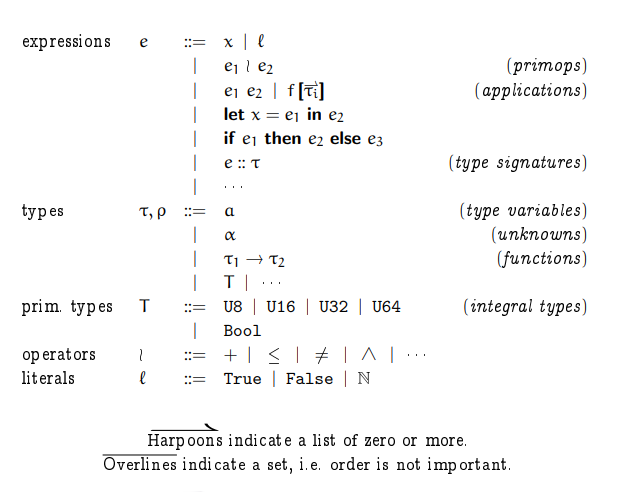
\includegraphics[width=350pt]{content/CogentGrammar.png}

    \begin{align*}
    \text{expressions}\quad e\; ::&= x\;\; |\;\; \ell & \text{(variables or literals)} \\
                &|\; e_1 \text{ \textasteriskcentered } e_2 & \text{(primitive operations)} \\
                &|\; e_1\; e_2 & \text{(function application)} \\
                &|\; \textbf{let } x = e_1 \textbf{ in } e_2 & \text{(let statements)} \\
                &|\; \textbf{if } e_1\; \textbf{ then } e_2 \textbf{ else } e_3 & \text{(conditional)} \\
                &|\; e_1\; e_2 & \text{(function application)} \\
                &|\; e_1 :: \tau & \text{(type signatures)} \\
                &|\; \dots \\
        \text{types}\quad \tau\; ::&= a & \text{(type variables)} \\
              &|\; \tau_1 \rightarrow \tau_2 & \text{(functions)} \\
              &|\; \mathcal{T} \\
              &|\; \dots \\
        \text{primitive types}\quad \mathcal{T}\; ::&= \textsc{ U8 } | \textsc{ U16 } | \textsc{ U32 } | \textsc{ U64 } |\; \textsc{Bool} \\
        \text{operators \ \ \ \textasteriskcentered }\; ::&= +\; |\; \leq\; |\; \geq\; |\; \neq\; |\; \dots \\
        \text{literals}\quad \ell\; ::&= \textsc{True } | \textsc{ False } |\; \mathbb{N}  \\
    \end{align*}

    \caption{The basic syntax for Cogent~\citep{ICFPCogent}}
    \label{fig:cogentGrammar}
\end{figure}

%%% Variant syntax
\begin{figure}
    \centering

    \begin{align*}
        \text{expressions}\quad e\; 
            ::&= \dots\; |\; \kappa\; e & \text{(variant constructor)} \\
              &|\; \textbf{case } e_1 \textbf{ of } \kappa\; e_2\; \dots & \text{(pattern matching)} \\
        \text{types}\quad \tau\;
            ::&= \dots\; |\; \langle \overline{\kappa^n\; \tau} \rangle & \text{(variant types)} \\
        \text{constructors}\quad \kappa
    \end{align*}

    \caption{The syntax for variant types within Cogent~\citep{ICFPCogent}}
    \label{fig:variantGrammar}
\end{figure}

%%% Record syntax
\begin{figure}
    \centering
    \begin{align*}
        \text{expressions}\quad e\; 
            ::&= \dots\; |\; \#\{\overline{f_i = e_i}\} & \text{(unboxed records)} \\
              &|\; \textbf{take } x\; \{ f = y\} = e_1 \textbf{ in } e_2 & \text{(record patterns)} \\
              &|\; \textbf{put } e_1.f = e_2 & \text{(record updates)} \\
              &|\; e_1.f & \text{(read record field)} \\
        \text{types}\quad \tau\;
            ::&= \dots\; |\; \{ \overline{f_i^n\; \tau_i} \} & \text{(variant types)} \\
        \text{field names } f
    \end{align*}
    \caption{The syntax for record types within Cogent~\citep{ICFPCogent}}
    \label{fig:recordGrammar}
\end{figure}



Cogent's uniqueness type system features a variety of basic types as well as the more advanced variants
and records.

\subsection{Primitive Types}

Cogent's primitive datatypes consist of Boolean types (\texttt{Bool}), and the four unsigned integer types \texttt{U8}, 
\texttt{U16}, \texttt{U32} and \texttt{U64}. Integer types can be upcast using the \texttt{\textsf{upcast}}
keyword to convert a smaller integer type into a larger one (e.g. a \texttt{U8} into a \texttt{U32}).
Details of these types can be seen in the syntax for Cogent's basic grammar in figure \ref{fig:cogentGrammar}.

Each of these primitive types are of fixed size, and thus are \emph{unboxed}, meaning they are stored on the
stack and are not linear variables.

Cogent also features \emph{tuples} (product types) through the standard tuple syntax across the ML
family of languages: $(a,b)$, and standard functions.

\subsection{Variant Types}

Cogent's variant types are inspired from the traditional sum types, where a variant type can contain
one of many specified types, the syntax for which is defined in \autoref{fig:variantGrammar}.

Consider the following example, we can reconstruct Haskell's \texttt{Maybe} type using our variants:

\begin{center}
    \textbf{type} \textit{Maybe} a = $\langle$ Nothing () $\vert$ Just a $\rangle$
\end{center}

Or a type to represent a choice of colours:

\begin{center}
    \textbf{type} \textit{RGB} = $\langle$ Red () $\vert$ Green () $\vert$ Blue () $\rangle$
\end{center}

Pattern matching on variants must be \textit{complete}, i.e. you must give a case for every possible constructor
of a variant, a constraint that helps keep functions total.

Variant types work well as a potential constructor for our recursive types. If we were to reference a
recursive parameter inside a variant type, we would be able to create a recursive structure as in Haskell.
However, as variants are \textit{unboxed} (stored on the fixed size stack), we cannot allow for dynamically sized structures
using only variants, so we must look elsewhere for a solution.

\subsection{Record Types}

Cogent's record types are objects that contain values via named fields. They come in two forms, \textit{boxed}
(stored dynamically on the heap) or \textit{unboxed} (stored statically in the stack). The syntax of both is
as in \autoref{fig:recordGrammar}.

For example, consider a record to bundle together user information:

\begin{center}
    \begin{tabular}{l}
    \textbf{type} \textit{User} = \{ \\
                    \hspace{1.5em} name: \texttt{String},\\
                    \hspace{1.5em} age: \texttt{U32}, \\
                    \hspace{1.5em} favouriteColour: \texttt{RGB}\\
                    \} \\
    \end{tabular}
\end{center}

Records allow for us to create dynamically sized objects, as we can used boxed records to chain together a
combination of records on the heap. With the aid of variant types, records can allow us to construct 
our recursive types with a recursive parameter, using variants to give the 
differing construction cases for the type.

\section{Termination And Recursive Types}

Proving total correctness about the programs we write is a very desirable result.
Computation performed by a program is useless if the program never returns the
result of the computation.
In a systems context, termination is especially desirable as an infinitely looping component of a
system could cause it to hang, denying services to other parts of a system which could be core to
system's function.

To deal with termination, we must consider the environment where we will prove termination for
Cogent programs, the Isabelle embedding, and how we can make this process easier on the type
level within Cogent.

\subsection{Proving Termination in Isabelle}


The official Isabelle tutorial~\citep{IsabelleTutorial} describes three methods of creating functions using
the keywords \textbf{primrec}, \textbf{fun} and \textbf{function}. The first, \textbf{primrec},
allows one to create a \textit{primitive recursive} function --- one that returns a constant or removes
a data type constructor from one of the arguments to the function in its body, `decreasing' in size every time.
These functions are total by construction, and therefore always terminate, removing the need of
an explicit termination proof (which is required to reason inductively about any Isabelle function.)
for all functions within Isabelle, unless they are defined to be partial, however as partial functions
may not terminate we do not want to consider them using them for our verification.
Primitive recursive functions however are limited in their expressiveness and are a subset of all computable
functions, so we cannot rely on them for the general case.

In his tutorial, Krauss~\citep{KraussIsabelle} discusses the details of the latter two of the three methods
of creating functions in Isabelle. The \textbf{fun} keyword instructs Isabelle to try and solve all necessary
termination proof obligations, rejecting the definition if it fails (either because the definition does not 
terminate or because Isabelle cannot prove it does alone). In contrast to \textbf{fun}, \textbf{function}
requires that the termination proofs be solved manually by whoever is writing the function.

% Perhaps another time :(
%\amos{Worth comparing the `gas' or `clock' approach as well, as used by CakeML (see CakeML: A Verified Implementation of ML, POPL 2014).
%There, the embedding of the program has an extra parameter which is a natural number describing how much time the program has to compute a result.
%At each recursive step, the clock is decremented, and if it reaches zero the program runs out of time and throws an exception.
%This lets you embed arbitrary programs as primitive recursion on a nat.
%You have to prove termination separately, but you can reason about the program assuming termination (assume that there exists a large enough clock that the program will return a valid value).}

Due to their automatic termination proofs, we would like as many Cogent functions as possible to be
primitive. For all others, we can achieve an embedding via \textbf{fun} to see if Isabelle can find
a termination proof for us, and as a last resort use \textbf{function} and have the proof writer
manually prove termination. 

\subsection{Strictly Positive Types}

Adding recursive types to a type system allows for expressions that are potentially infinitely recursive,
as discussed by Wadler~\cite{RecursiveTypesForFree}, who explains the potential for recursive expressions
to cause non-termination through polymorphic lambda calculus. In his paper, he discusses how this
quality can be qualified with positive and negative data types.

Suppose a data type in its general form $T$ and its data constructors $C_{1..n}$, each with a number of arguments 
$\tau_{i1}..\tau_{ik}$:

\begin{center}
    \begin{tabular}{l}
        $T = C_1\; \tau_{11} \; \tau_{12} \; \dots$ \\
        $\hspace{1.5em} \vert\; C_2\; \tau_{21} \; \tau_{22} \; \dots$ \\
        $\hspace{1.5em} \vert\; \dots$ \\
    \end{tabular} 
\end{center}

\theoremstyle{definition}
\begin{definition}
    A data type $T$ is said to be in a \textit{negative position} if $T$ appears nested as an argument
    to a function an odd amount of times inside any $\tau_{ij}$, and said to be in a \textit{positive position}
    if $T$ appears nested as an argument to a function an even amount of times inside $\tau_{ij}$.
\end{definition}

\theoremstyle{definition}
\begin{definition}
    A data type $T$ is a \textit{negative} data type if it appears in a negative position 
    in one of its constructors.
\end{definition}

\theoremstyle{definition}
\begin{definition}
    A data type $T$ is a \textit{positive} data type if only appears nested in a positive position
    in all of its constructors.
\end{definition}

In simpler terms, if $T$ appears to the left of a function arrow an odd amount of times, it is negative and if
to the left an even amount of times then it is positive.

For example:

\begin{center}
    \begin{tabular}{l}
        $E = C\; (\underline{E} \rightarrow E)$ \\
        $K = D\; (\underline{(\underline{K} \rightarrow_1 Int)} \rightarrow_2 K)$
    \end{tabular} 
\end{center}

Here, the data type $E$ is negative as it appears in a negative position (denoted here by an underline)
to a function in the first argument of $C$.
$K$ however is positive as it appears only ever in a positive position as it is nested as an argument
in function 1 ($\rightarrow_1$) and again in function 2 ($\rightarrow_2$) for a total of two times.

Allowing for negative types in our system allows for data structures that are infinitely recursive,
which if iterated over would potentially cause non-termination. Consider
the following example in \textsc{Haskell}:

\begin{center}
    \begin{tabular}{l}
            \textbf{data} \textsf{Bad = A (Bad $\rightarrow$ Bad)} \\ \\

            \textsf{g :: Bad $\rightarrow$ Bad} \\
            \textsf{g (A f) = f (A f)} \\ \\

            \textsf{infiniteExpression = g (A g)}
    \end{tabular} 
\end{center}

By our definition, we can see that our type \textit{Bad} is a \textit{negative} type and using it we were able
to construct the infinitely recursive expression, \textsf{g (A g)}
This is not an issue in Haskell due to its lazy evaluation and Haskell allows its programmers to write
infinite loops freely, however in Cogent these expressions would be detrimental to our termination
proofs as iterating over them potentially results in non-termination, and in this
situation will hang when \textit{infiniteExpression} is constructed.
Although this example was constructed artificially, situations may arise where
programmers may accidentally construct such an expression, so we must seek a way to
eliminate them from our language.

Many theorem provers and dependently typed languages make use of \textit{strictly positive} types, which
prohibit the construction of infinitely recursive data structures, that under a dependant type system
both negative and simple positive types allow.
\textsc{Agda}\citep{AgdaStrictlyPositive}, \textsc{Coq}\citep{CoqStrictlyPositive} and even
Isabelle\citep{IsabelleStrictlyPositive} feature this exact constraint, as allowing for negative
or non-strictly positive types introduce logical inconsistencies which can be used to prove false statements,
something that is unacceptable for a theorem prover.

The definition of strictly positive is discussed by Conquand and Paulin~\citep{CoquandTypes}, and is as follows:

\theoremstyle{definition}
\begin{definition}
    \label{def:sp}
    Given a data type $T$ and its constructors $C_{1..n}$, for every argument $\tau_{ij}$
    of any data constructor $C_i$ where $\tau_{ij}$ is a function, $T$ is said to be \textit{strictly positive} if 
    $T$ does not occur as an argument to any $\tau_{ij}$:

    \begin{center}
        $\forall\; \tau_{ij}.\;
        (\tau_{ij} = \phi_{1} \rightarrow \dots \rightarrow \phi_{k})
        \implies T \notin \phi_{1..k-1}$
    \end{center}
\end{definition}

Strictly positive types can also be defined as types where $T$ appears in a negative or positive 
position exactly zero times (i.e. it does not appear to the left of any arrow).

In their paper, Conquand and Paulin further discuss the ability to produce an \textit{eliminator} or a
\textit{fold} from any strictly positive type, which corresponds to an induction principle on the type.

Consider a type for natural numbers with two constructors for zero and successor:

\begin{center}
    \begin{tabular}{l}
        $Nat = \textsc{Z}\; \vert\; \textsc{S}\; Nat$ \\
    \end{tabular} 
\end{center}

We can see $Nat$ is a strictly positive type and the induction principle it produces
for any predicate over natural numbers, $P$, is:

\[
    \infer{
        \forall(N : Nat).\;\; P(N)
    }{
        P(Z) \quad & \forall (X : Nat).\; P(X) \implies P(S\; X)
    }
\]

Where in order to prove our predicate $P$, we prove it for each case of how our type $T$ could have been
constructed, which each constructor for our our type supplies.
That is, to prove any predicate $P$ inductively over nats ($\forall(N : Nat).\; P(N)$)
we prove it for the base (zero) case $P(Z)$ and then assuming the predicate holds
for a natural number $X$, we prove it for its successor case $S\; X$: $P(X) \implies P(S\; X)$.

The interactive theorem prover Isabelle generates the same induction principle for any type created in
Isabelle. We can get the same induction principle over natural numbers by redefining our $Nat$
type in Isabelle, as in figure \ref{fig:IsabelleNatInduct}.

\begin{center}
    \begin{figure}
        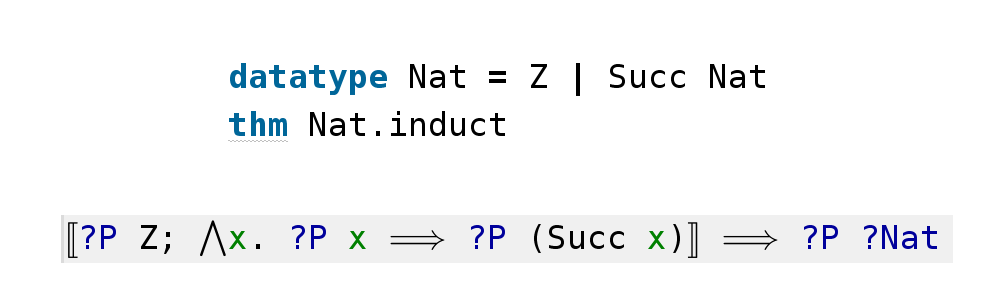
\includegraphics[width=\linewidth]{content/isabelleNatInduct.png}
        \caption{A type for natural numbers defined in Isabelle, and the generated 
        induction principle associated with the type.}
        \label{fig:IsabelleNatInduct}
    \end{figure}
\end{center}

\FloatBarrier

Considering our Cogent embedding will be within Isabelle, if we can embed our native
Cogent types into an Isabelle type then we gain Isabelle's automatically generated
induction principle over our Cogent types, allowing for much 
simpler reasoning about our Isabelle embedding.

\section{Linear And Uniqueness Types}

Linear types are a kind of substructural type system as discussed by Walker~\citep{Substructural}.
Many standard programming languages such as \textsc{C}, \textsc{Java} and \textsc{Haskell} feature
three standard structural typing rules, described in figure \autoref{def:structural}.

\begin{figure}
    \centering
    $$
        \infer[Exchange]{
            \Gamma_1\Gamma_2 \vdash e : \tau
        }{
            \Gamma_2\Gamma_1 \vdash e : \tau
        }\quad
        \infer[Weakening]{
            \Gamma_1\Gamma_2 \vdash e : \tau
        }{
            \Gamma_1 \vdash e : \tau
        }\quad
        \infer[Contraction]{
            \Gamma_1\Gamma_2 \vdash e : \tau
        }{
            \Gamma_1\Gamma_1\Gamma_2 \vdash e : \tau
        }
    $$
    \caption{Structural typing rules}
    \label{def:structural}
\end{figure}

\textit{Exchange} is the rule that states that the order in which we add variables in an environment
is irrelevant. A conclusion of this is that if a term $e$ typechecks under environment $\Gamma$,
then any permutation of $\Gamma$ will also typecheck $e$.

\textit{Weakening} states that if a term $e$ typechecks under the assumptions
in $\Gamma_1$, then $e$ will also typecheck if extra assumptions are added to the environment.

\textit{Contraction} states that if we can typecheck a term $e$ using two identical
assumptions, then we are able to check $e$ with just one of those two assumptions.

Substructural type systems however control access to information within the program by limiting which
of the structural typing rules are allowed under certain contexts. Linear types ban the use of the
contraction and weakening rules, which has the consequence that all linear variables must be used 
at least once (by lack of weakening) and at most once (by lack of contraction), hence exactly one time.

One powerful benefit that linear types allow is \textit{static allocation} of objects, which Cogent
features. Predicting when an object in a program will be last used (and after deallocated)
is undecidable as it is a nontrivial semantic property by Rice's Theorem~\citep{Sipser},
however a linear type system can make it possible to deallocate this memory after its first use
by the use once rule. The result is a langauge that does not require a garbage collector,
can check that programs appropriately handle allocated resources statically as this can now
be determined statically.

Wadler~\citep{LinearTypesChangeTheWorld} also describes the performance benefits of destructive updates
that linear types potentially grant. As we have a guarantee that no other part of a program is
referencing a particular object (variables must be used exactly once), when performing
an operation on an object, the resultant object can be our old object with the result
of our operation performed in place (i.e. destructively mutated).

Consider the following program in Java:

\lstinputlisting[language=Java,basicstyle=\small]{content/destructive.java}

In this example we attempt to double a copy of a list of numbers in place by use of the \verb|doubleNumbers|
function on \verb|copyOfNumbers|, however by updating it in place has changed the original variable outside
the function \verb|oldNumbers|. If a programmer mistakenly uses \verb|oldNumbers| again without realising that
\verb|doubleNumbers| has mutated it instead of a copy of it, it would most likely cause an error. In 
Java this kind of destructive update cannot be done safely whilst \verb|oldNumbers| still exists, and we
must resort to copying.

Linear types prevent this kind of mistake, as the duplicate reference that
\verb|oldNumbers| and \verb|copyOfNumbers| share would be eliminated once \verb|oldNumbers| is used once,
which in turn allows for a destructive update on \verb|oldNumbers| to take place with the result stored in
copyOfNumbers.

Wadler however shows that mere linearity is not enough to guarantee safe destructive updates, as nonlinear
variables with multiple references may be cast to linear ones, breaking the single reference guarantee
for linear types. This is from the result that adding typecasting to and from linear variables grants 
controlled access to the contraction and weakening rules that linear types explicitly prohibit.

He further discusses seperately~\citep{WadlerLinearLogic} that with the removal of
the ability to perform such an action, one can gain the \textit{uniqueness} types that Cogent 
exibits. With uniqueness types, it is truly impossible for linear variables to have multiple references,
and thus destructive updates on these variables are safe. 

All boxed types in Cogent are linear, and therefore must have at most one reference to each,
however unboxed objects are only linear if they contain other linear values.
With our implementation of recursive types, we must consider maintaining the linear and uniqueness constraints
that Cogent features, and create these types in such a way that they integrate nicely with the existing
system.